\section{Evaluation}

\subsection*{Benchmarks}
\label{sec:benchmarks}
We choose five application kernels to characterize from Phoenix -- a shared memory implementation of Google's MapReduce model. These workloads represent computations from domains amenable to approximations e.g., image processing and machine learning. The following breifly details each benchmark used in the evaluation. 

\textbf{Histogram} counts the frequency of RGB value occurances per pixel from a range of 0-255. The application divides the image into sections and computes histograms on each part seperately. Seperate histograms are reduced into a single, total histogram once all parallel computations are complete. Error-tolerant features of the application can include loading/storing of the pixel data. Small deviations in the frequency of occurances in the range from 0-255 are likely to go unnoticed. For the evaluation we use a 100MB bitmap as the input. 

\textbf{KMeans} implements an iteration of the iterative convergence kmeans clustering algorithm. The algorithm consists of a cluster assignment step and an update step. Cluster assignment takes a subset of the input data points and assigns them to appropriate "nearest" clusters, i.e., having the least squared Euclidean distance. The update step calculates the new means of each cluster for the next iteration of the algorithm. Error-tolerant computions may include the calculations of the Euclidean distance in the cluster assignment step, and the mean for each cluster in the update step. For the evaluation we use an input of 10000 data points.

\textbf{Linear Regression} Something... Input size of 100MB.

\textbf{Matrix Multiply} Something... Multiplies two matrices of size 500x500

\textbf{PCA} implements a segment of the Principal Component Analysis algorithm, namely the mean and covariance calculations. The input is a matrix of pseudo-randomly generated points. The mean calculation paralellizes the generation of the mean vector by computing on subsets of the input matrix rows. The covariance calculates portions of the covariance matrix in parallel given a subset of data. Both mean and convariance computations are amenable to approximation. For the evaluation we use an 1000x1000 matrix as the input.

\subsection*{Simulator}

gem5 simulator. The simulated machine is described in Table: \ref{tab:machine_config}

\begin{table}[htbp]
\caption{Simulated Machine Configuration}
	\begin{center}
		\begin{tabular}{|c|c|}
			\hline

			\textbf{Parameter} & \textbf{Values}\\
			\hline

			Cores & 8 Cores, X86, In-order, Atomic Memory Accesses\\
			\hline

			L1 & \makecell{Private 64kB DCache/32kB ICache, \\ 2-Way Set Assoc., 64B Block, Pseudo-LRU}\\
			\hline

			L2 & \makecell{Private Unified 1MB, 8-Way Set Assoc., \\ 64B Block, Pseudo-LRU}\\
			\hline

			L3 / LLC & \makecell{Shared 20MB, 16-Way Set Assoc., \\ 64B Block, Pseudo-LRU}\\
			\hline

			Coherence & Directory MESI Protocol\\
			\hline

		\end{tabular}
	\label{tab:machine_config}
	\end{center}
\end{table}


\subsection*{Coherence Misses}

Coherence Misses are defined as misses due to the cache line being in the wrong coherence state, i.e., the tag is found in the cache, but the cache access is a store on a read-only/invalid line, or a load on an invalid line, resulting in a miss.

Observations on the amount of coherence misses seen in Figures \ref{fig:L1_misses} and \ref{fig:L2_misses}.

\begin{enumerate}
	\item The ratio of cache misses to cache accesses is higher in the L2 cache, many of which are due to coherence misses. Possibly because the L2 cache is larger, and is able to hold more cache lines in read-only/invalid coherence states for stores/loads to miss on.
	\item A considerable chunck of the coherence misses (seen in the (c) subfigures) are from stores. Although most of them are from loads, implementing SAS might decrease misses from subsequent loads.
	\item Matrix Multiply benchmark performs well in that there are very little cache misses, not just coherence misses. Input matrices are partitioned onto threads with little migrating data (seems to be only a published data type of sharing, one parent and multiply readers) and the computions seem to have good spatial locality which might explain why we see little misses.
	\item PCA shows minor amount of misses in the L1, a substantial amount in the L2, neither of which are due to misses on wrong coherence states. This could be due to the calculation of the covariance matrix. The algorithm reads from the matrix of points and a matrix of means to calculate the covariance. Since both matrices are large enough to overflow the L2 and accesses its elements has a long distance in address space, this could be the reason the L2 sees a lot of misses. Not to sure why L1 doesn't generate a lot of misses.
	\item Linear Regression sees high amount of coherence traffic, specifically from false sharing due to the \texttt{lreg\_args} structure. Array \texttt{tid\_args} of \texttt{lreg\_args} in the main thread passes each \texttt{lreg\_args} to the compute threads. However the structures may not be aligned to the cache block which would result in false sharing since the compute threads read and modify \texttt{lreg\_args} \cite{Liu:2011, Liu:2014}.
	\item Histogram has similar behaviour to Linear Regression due to a shared heap structure \texttt{thread\_arg\_t}. Each compute thread's \texttt{thread\_arg\_t} structure may not be aligned to the cache line causing false sharing while the threads are reading and modifying \cite{Liu:2014}.
\end{enumerate}

\begin{figure*}[htbp]
	\begin{subfigure}{0.33\textwidth}
		\centering
		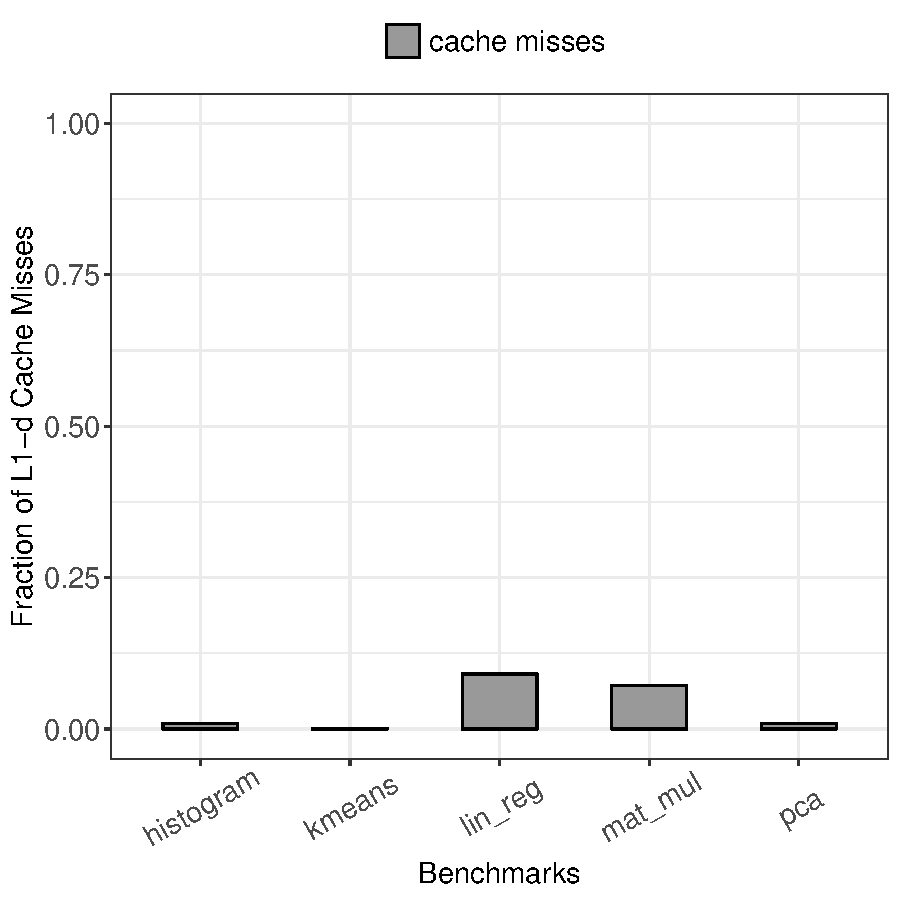
\includegraphics[scale=0.4]{graphs/cache_misses_L1.pdf}
		\caption{Fraction of cache accesses that resulted in misses on the L1-d.}
	\end{subfigure}
	% Need a space between subfigures
	\begin{subfigure}{0.33\textwidth}
		\centering
		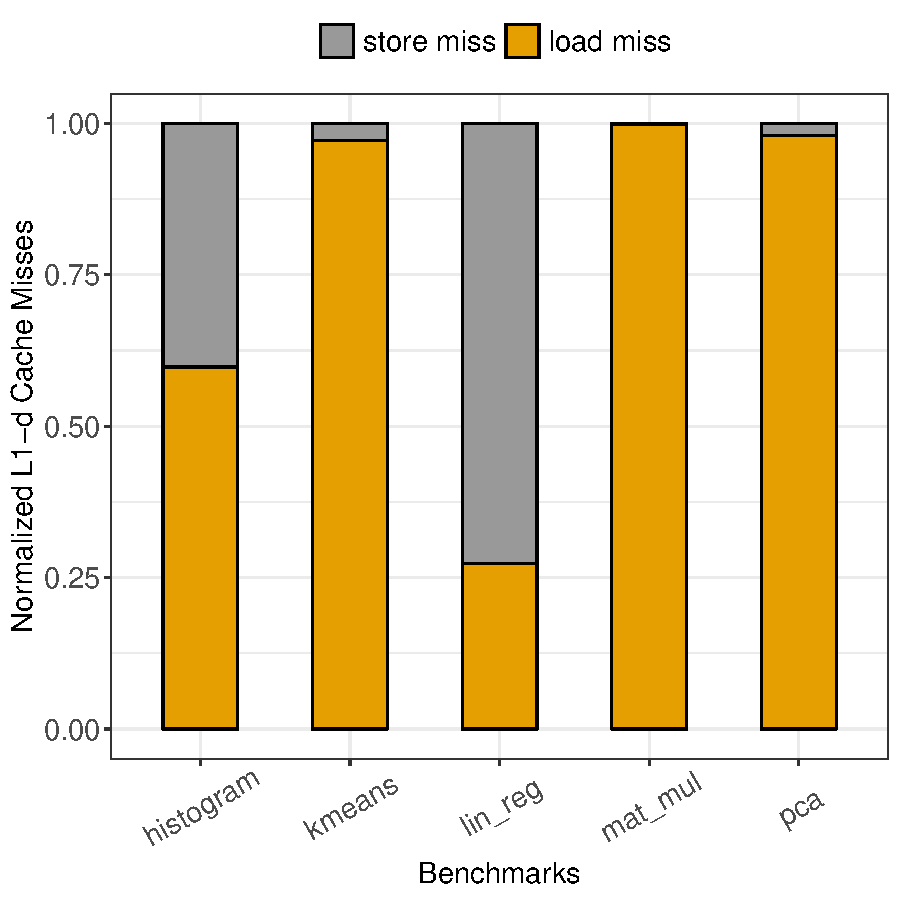
\includegraphics[scale=0.4]{graphs/all_misses_L1.pdf}
		\caption{Breakdown of all L1-d cache misses into misses on loads or stores.}
	\end{subfigure}
	% Need a space between subfigures
	\begin{subfigure}{0.33\textwidth}
		\centering
		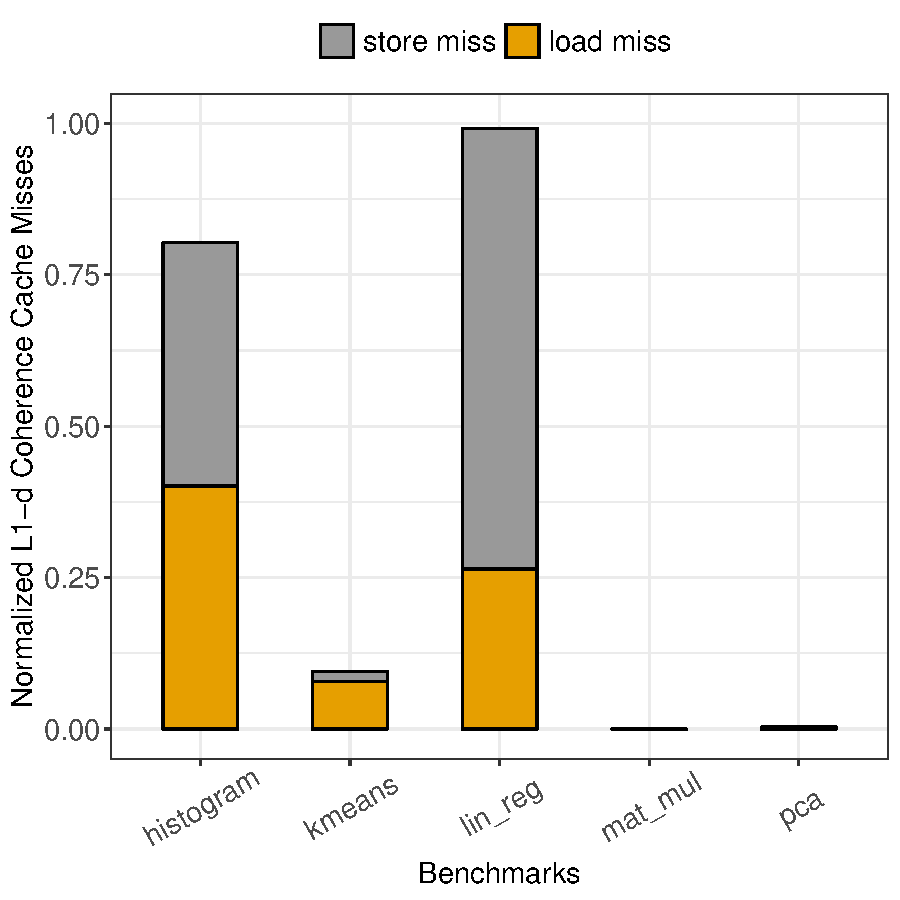
\includegraphics[scale=0.4]{graphs/coherence_misses_L1.pdf}
		\caption{Breakdown of the L1-d cache misses into load misses or store misses due to coherence state. Misses that are not shown are due to capcity and conflict misses.}
	\end{subfigure}
\caption{} %need this for label to ref properly
\label{fig:L1_misses}
\end{figure*}




\begin{figure*}[htbp]
	\begin{subfigure}{0.33\textwidth}
		\centering
		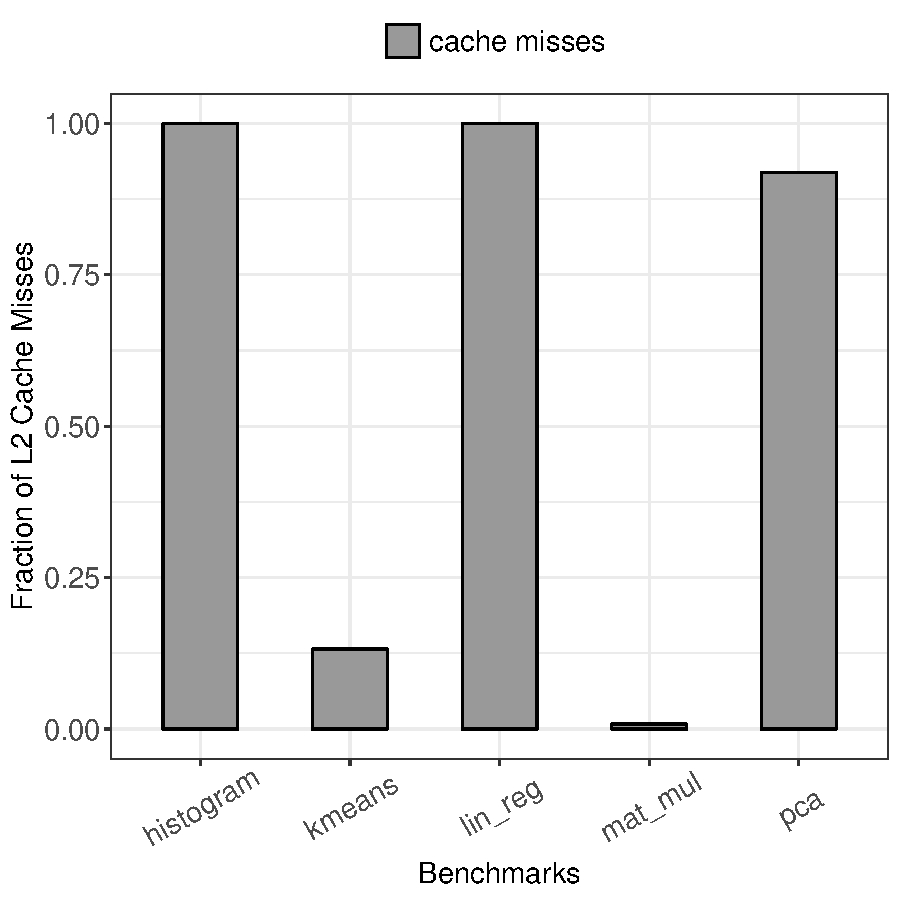
\includegraphics[scale=0.4]{graphs/cache_misses_L2.pdf}
		\caption{Fraction of cache accesses that resulted in misses on the L2.}
	\end{subfigure}
	% Need a space between subfigures
	\begin{subfigure}{0.33\textwidth}
		\centering
		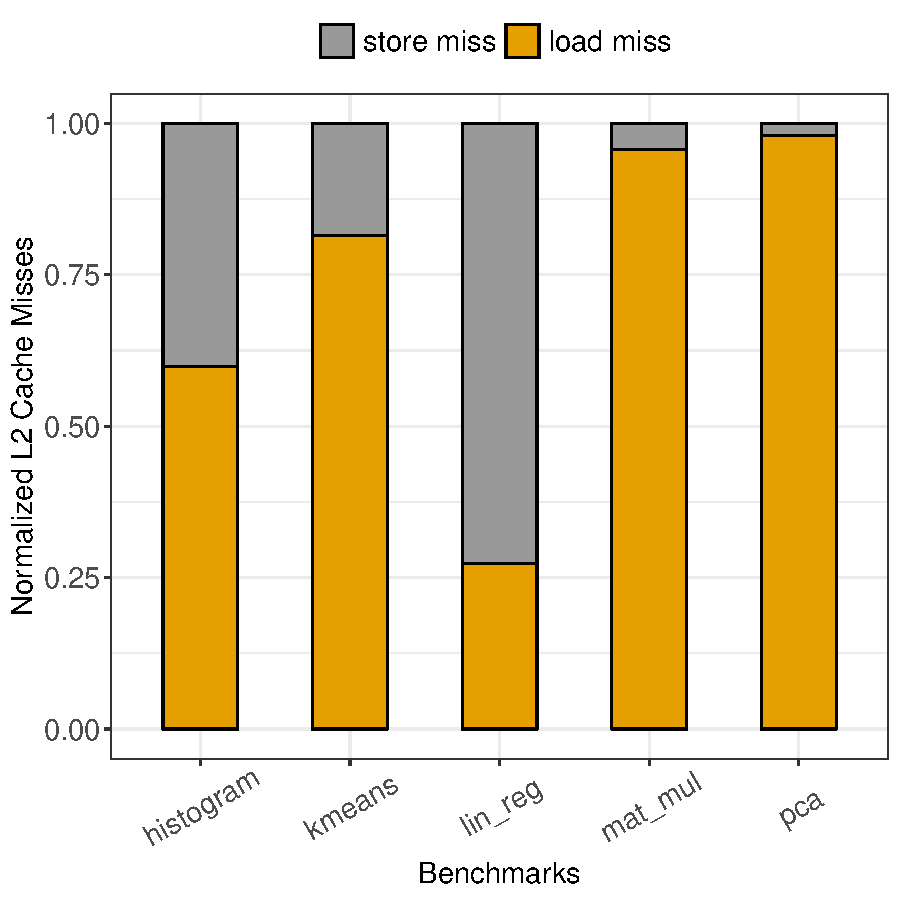
\includegraphics[scale=0.4]{graphs/all_misses_L2.pdf}
		\caption{Breakdown of all L2 cache misses into misses on loads or stores.}
	\end{subfigure}
	% Need a space between subfigures
	\begin{subfigure}{0.33\textwidth}
		\centering
		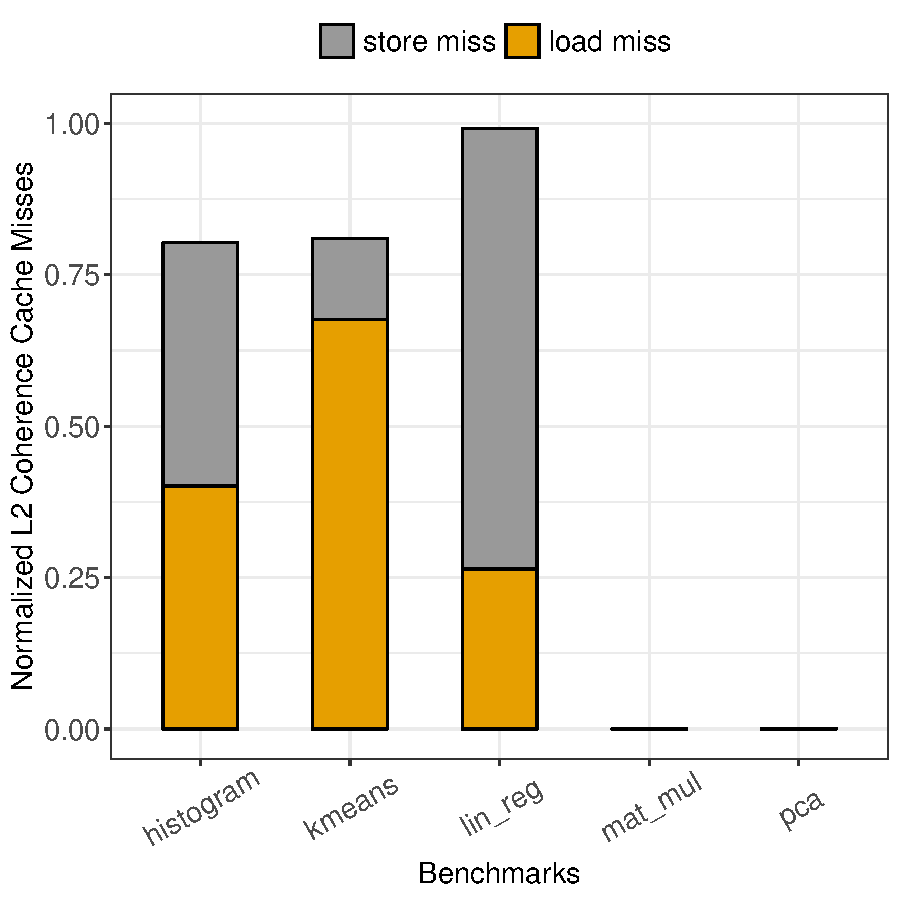
\includegraphics[scale=0.4]{graphs/coherence_misses_L2.pdf}
		\caption{Breakdown of the L2 cache misses into load misses or store misses due to coherence state. Misses that are not shown are due to capcity and conflict misses.}
	\end{subfigure}
\caption{} %need this for label to ref properly
\label{fig:L2_misses}
\end{figure*}


\subsection*{Store-Value Similarity}


Benchmark Histogram -- shown in Figures \ref{fig:histogram_valsim} and \ref{fig:histogram_valsim_top5}

Benchmark KMeans -- shown in Figures \ref{fig:kmeans_valsim} and \ref{fig:kmeans_valsim_top5}

Benchmark Linear Regression -- shown in Figures \ref{fig:linear_regression_valsim} and \ref{fig:linear_regression_valsim_top5}

Benchmark Matrix Multiply -- shown in Figures \ref{fig:matrix_multiply_valsim} and \ref{fig:matrix_multiply_valsim_top5}

Benchmark PCA -- shown in Figure \ref{fig:pca_valsim_top5}. Since there were many unique approximatable addresses to process for this benchmark, processing the results for all of them took a long time. I only show the results for the top 5 traffic generating stores


\begin{table*}[htbp]
\caption{Store-value similarity for all approximatable stores.}
	\begin{center}
		\begin{tabular}{|c|c|c|c|c|c|c|c|}
			\hline
			% \textbf{Table}&\multicolumn{3}{|c|}{\textbf{Table Column Head}} \\
			% \cline{2-4} 
			\textbf{Benchmark} & \textbf{\# Stores Sampled}& \textbf{\# Unique Addresses} & \textbf{Median} & \textbf{Mean} & \textbf{Std. Dev.} & \textbf{Max} & \textbf{Min} \\
			\hline

			\textbf{Histogram} & $1.04\times10^9$ & 5142 & 241 & 1162.15 & $5.90 \times 10^6$ & $1.68 \times 10^9$ & $-2.1 \times 10^9$\\
			\hline

			\textbf{KMeans} & $193\times10^6$ & 1440 & 7 & $-449 \times 10^6$ & $904 \times 10^6$ & $2.1 \times 10^9$ & $-2.1 \times 10^9$\\
			\hline

			\textbf{Linear Regression} & $773\times10^6$ & 40 & -2 & 240.89 & $793 \times 10^3$ & $2.1 \times 10^9$ & $-2.1 \times 10^9$\\
			\hline

			\textbf{PCA} & $502\times10^6$ & 428290 & -99 & $-3.91 \times 10^6$ & $92.1 \times 10^6$ & $1.7 \times 10^9$ & $-2.1 \times 10^9$\\
			\hline

			\textbf{Matrix Multiply} & $159\times10^6$ & 8 & 78 & $-3.30 \times 10^6$ & $84.9 \times 10^6$ & $1.68 \times 10^9$ & $-2.1 \times 10^9$\\
			\hline

		\end{tabular}
	\label{tab:val_sim}
	\end{center}
\end{table*}

\begin{table*}[htbp]
\caption{Store-value similarity for top 5 traffic generating approximatable stores.}
	\begin{center}
		\begin{tabular}{|c|c|c|c|c|c|c|c|}
			\hline
			% \textbf{Table}&\multicolumn{3}{|c|}{\textbf{Table Column Head}} \\
			% \cline{2-4} 
			\textbf{Benchmark} & \textbf{\# Stores Sampled}& \textbf{\# Unique Addresses} & \textbf{Median} & \textbf{Mean} & \textbf{Std. Dev.} & \textbf{Max} & \textbf{Min} \\
			\hline

			\textbf{Histogram} & $35.4\times10^5$ & 5 & -1 & 483.07 & $1.09 \times 10^6$ & $1.68 \times 10^9$ & $-2.1 \times 10^9$\\
			\hline

			\textbf{KMeans} & $3.75\times10^6$ & 5 & 0 & $-320 \times 10^6$ & $790 \times 10^6$ & $2.1 \times 10^9$ & $-2.1 \times 10^9$\\
			\hline

			\textbf{Linear Regression} & $136\times10^6$ & 5 & -1 & 156.92 & $752 \times 10^3$ & $2.1 \times 10^9$ & $-2.1 \times 10^9$\\
			\hline

			\textbf{PCA} & $313\times10^6$ & 5 & -1 & $-2.19 \times 10^6$ & $68.7 \times 10^6$ & $1.7 \times 10^9$ & $-2.1 \times 10^9$\\
			\hline

			\textbf{Matrix Multiply} & $113\times10^6$ & 5 & 20 & $-2.92 \times 10^6$ & $80.0 \times 10^6$ & $1.68 \times 10^9$ & $-2.1 \times 10^9$\\
			\hline

		\end{tabular}
	\label{tab:val_sim_top5}
	\end{center}
\end{table*}


\begin{figure*}[htbp]
	\begin{subfigure}{0.33\textwidth}
		\centering
		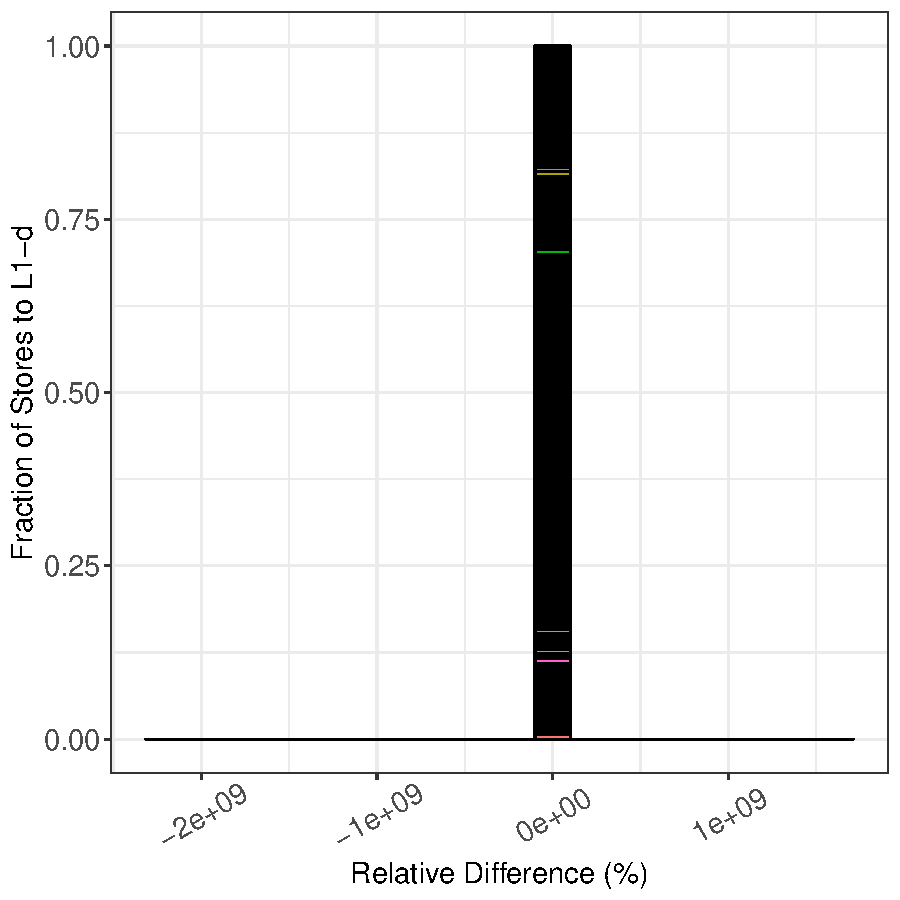
\includegraphics[scale=0.4]{graphs/histogram/full_hist.pdf}
		\caption{Histogram of the fraction of approximateable stores within a store-value relative difference. Shown is the full realtive difference range.}
	\end{subfigure}
	% Need a space between subfigures
	\begin{subfigure}{0.33\textwidth}
		\centering
		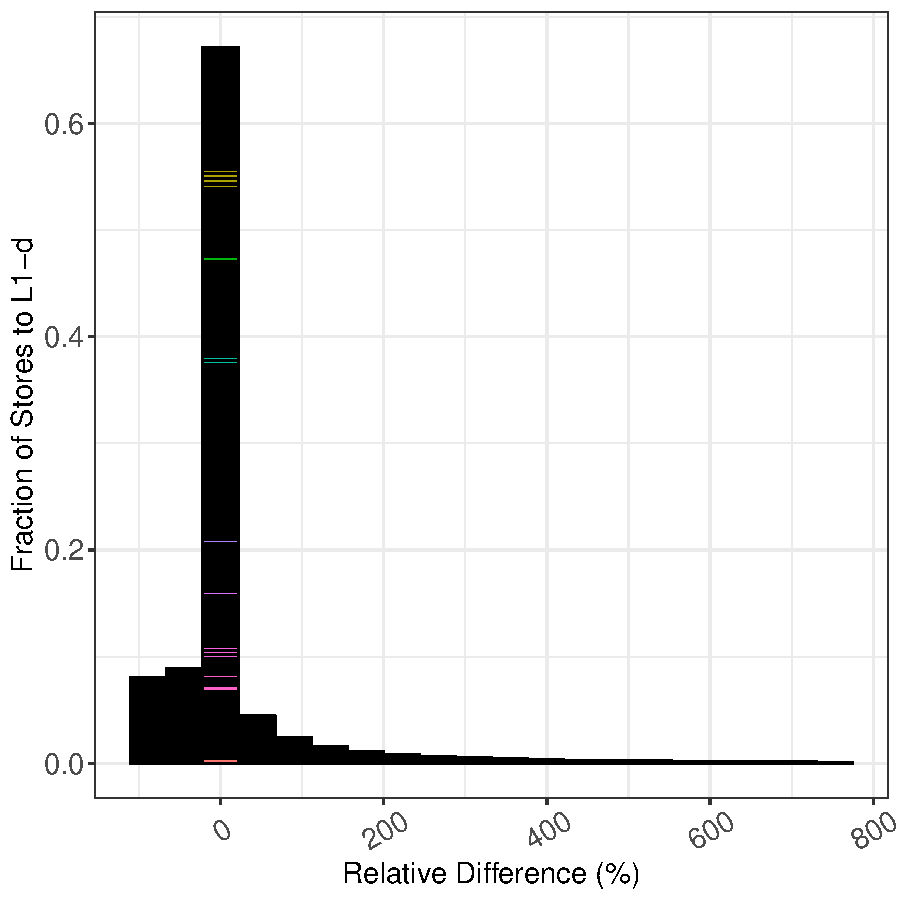
\includegraphics[scale=0.4]{graphs/histogram/narrow_hist.pdf}
		\caption{Histogram of the fraction of approximateable stores within a store-value relative difference. Shown is focused view between relative percent difference of -500\% and 500\%.}
	\end{subfigure}
	% Need a space between subfigures
	\begin{subfigure}{0.33\textwidth}
		\centering
		\includegraphics[scale=0.4]{graphs/histogram/narrow_dist.pdf}
		\caption{Density of the fraction of approximateable stores within a store-value relative difference. Shown is focused view between relative percent difference of -500\% and 500\%.}
	\end{subfigure}

\caption{Histogram}
\label{fig:histogram_valsim}%
\end{figure*}

\begin{figure*}[htbp]
	\begin{subfigure}{0.33\textwidth}
		\centering
		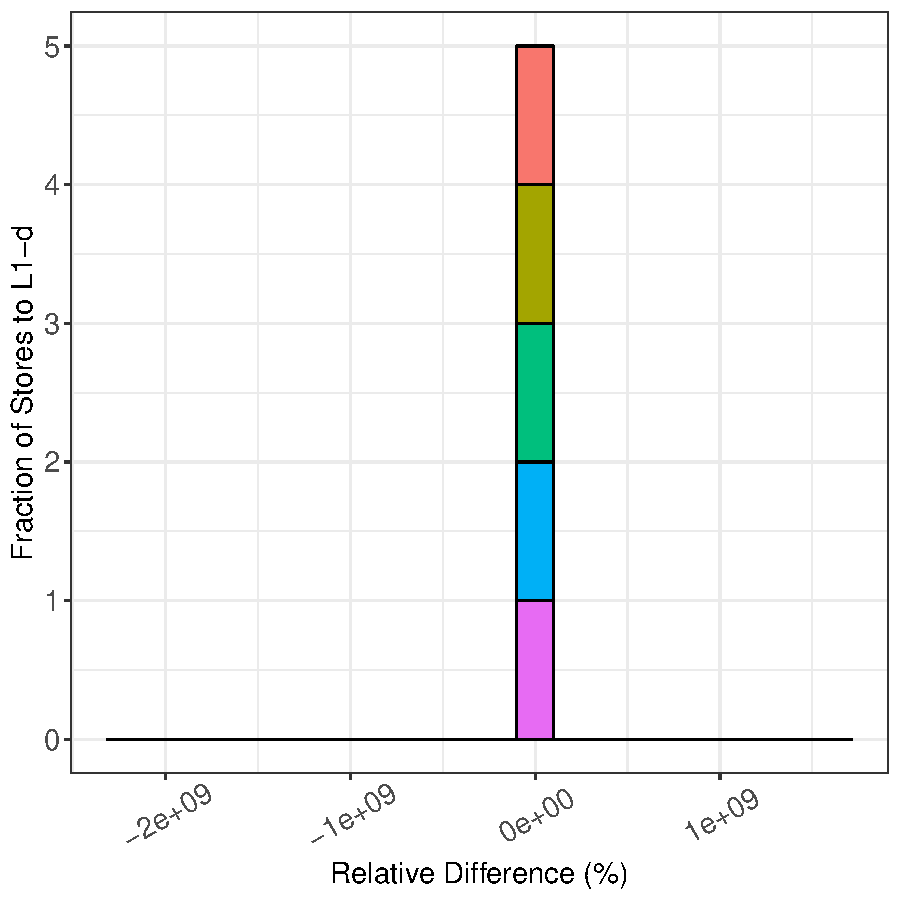
\includegraphics[scale=0.4]{graphs/histogram_top5/full_hist.pdf}
		\caption{Histogram of the fraction of approximateable stores within a store-value relative difference. Shown is the full realtive difference range.}
	\end{subfigure}
	% Need a space between subfigures
	\begin{subfigure}{0.33\textwidth}
		\centering
		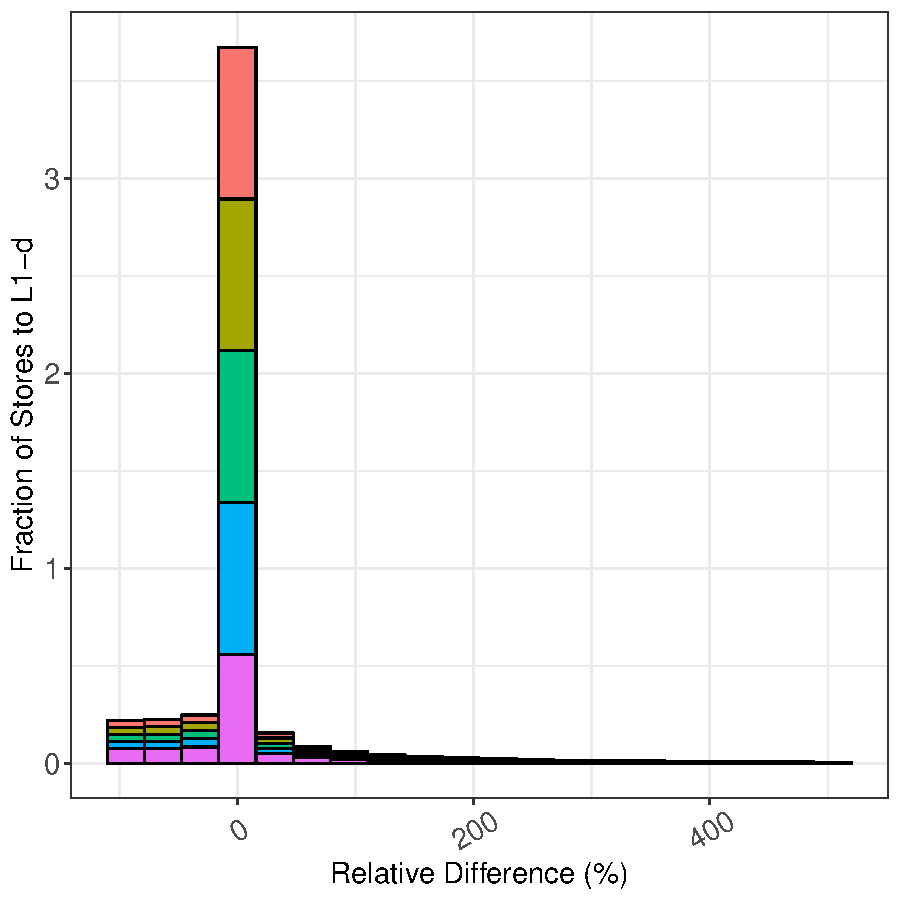
\includegraphics[scale=0.4]{graphs/histogram_top5/narrow_hist.pdf}
		\caption{Histogram of the fraction of approximateable stores within a store-value relative difference. Shown is focused view between relative percent difference of -500\% and 500\%.}
	\end{subfigure}
	% Need a space between subfigures
	\begin{subfigure}{0.33\textwidth}
		\centering
		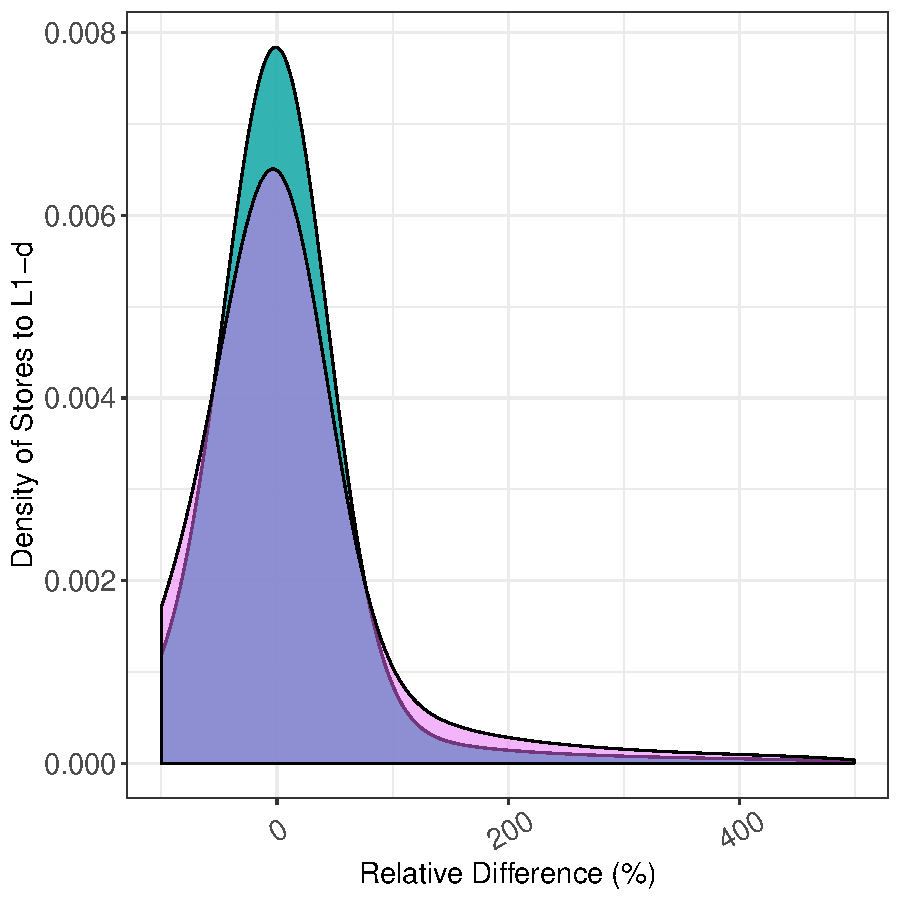
\includegraphics[scale=0.4]{graphs/histogram_top5/narrow_dist.pdf}
		\caption{Density of the fraction of approximateable stores within a store-value relative difference. Shown is focused view between relative percent difference of -500\% and 500\%.}
	\end{subfigure}
\caption{Histogram top 5 stores} %need this for label to ref properly
\label{fig:histogram_valsim_top5}
\end{figure*}

\begin{table}[htbp]
\caption{Stores saved for different level of approximations for benchmark Histogram}
	\begin{center}
		\begin{tabular}{|c|c|}
			\hline

			\textbf{Relative Difference (\%)} & \textbf{Stores Saved (\%)}\\
			\hline

			\textbf{1} & 58.02\\
			\hline

			\textbf{5} & 68.62\\
			\hline

			\textbf{10} & 71.16\\
			\hline

			\textbf{20} & 74.33\\
			\hline

			\textbf{30} & 76.97\\
			\hline

			\textbf{40} & 79.40\\
			\hline

			\textbf{50} & 81.78\\
			\hline

		\end{tabular}
	\label{tab:histogram_reldiff}
	\end{center}
\end{table}

\begin{figure*}[htbp]
	\begin{subfigure}{0.33\textwidth}
		\centering
		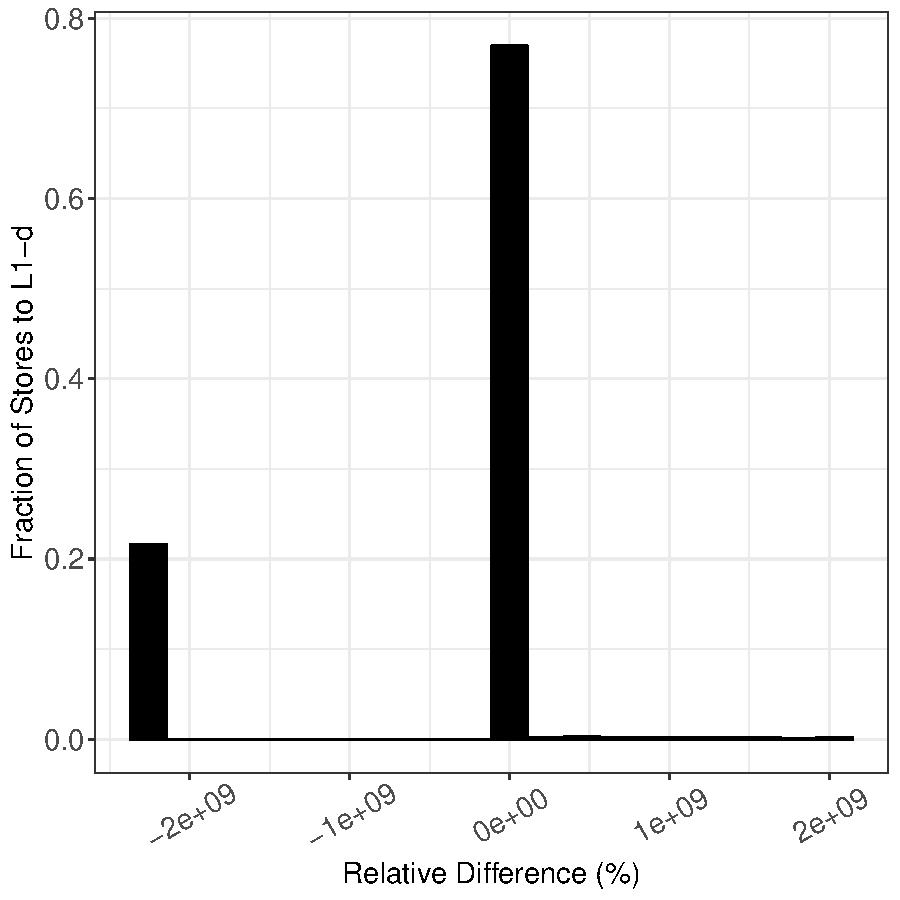
\includegraphics[scale=0.4]{graphs/kmeans/full_hist.pdf}
		\caption{Histogram of the fraction of approximateable stores within a store-value relative difference. Shown is the full realtive difference range.}
	\end{subfigure}
	% Need a space between subfigures
	\begin{subfigure}{0.33\textwidth}
		\centering
		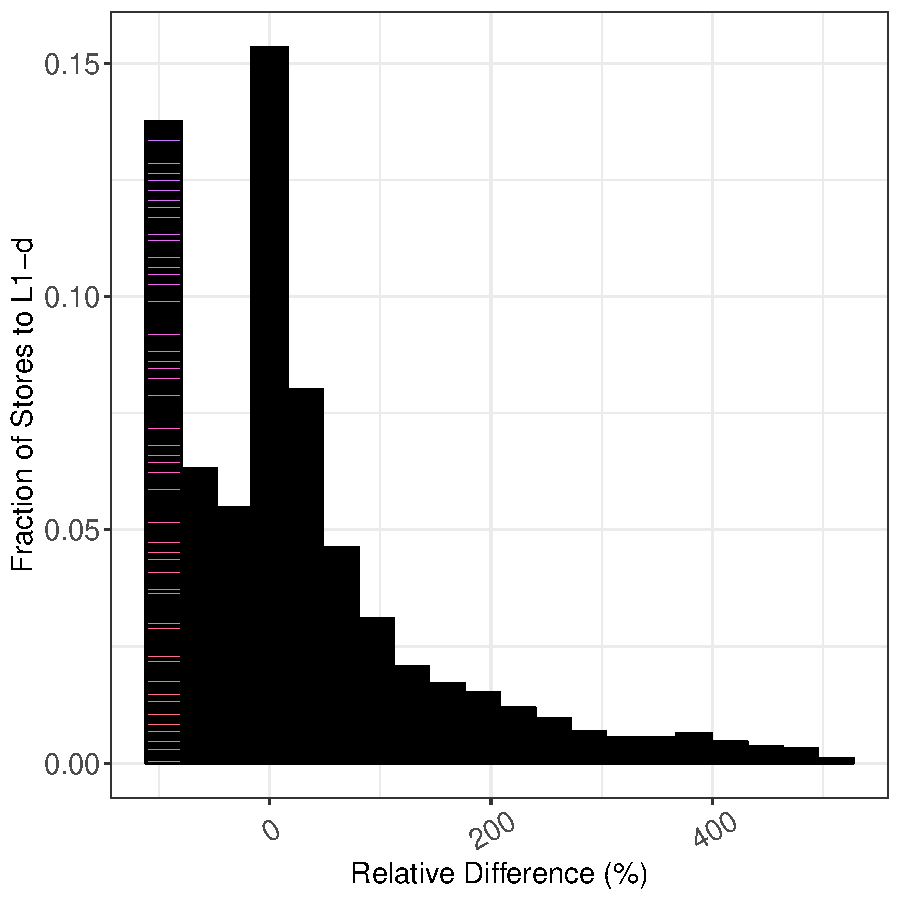
\includegraphics[scale=0.4]{graphs/kmeans/narrow_hist.pdf}
		\caption{Histogram of the fraction of approximateable stores within a store-value relative difference. Shown is focused view between relative percent difference of -500\% and 500\%.}
	\end{subfigure}
	% Need a space between subfigures
	\begin{subfigure}{0.33\textwidth}
		\centering
		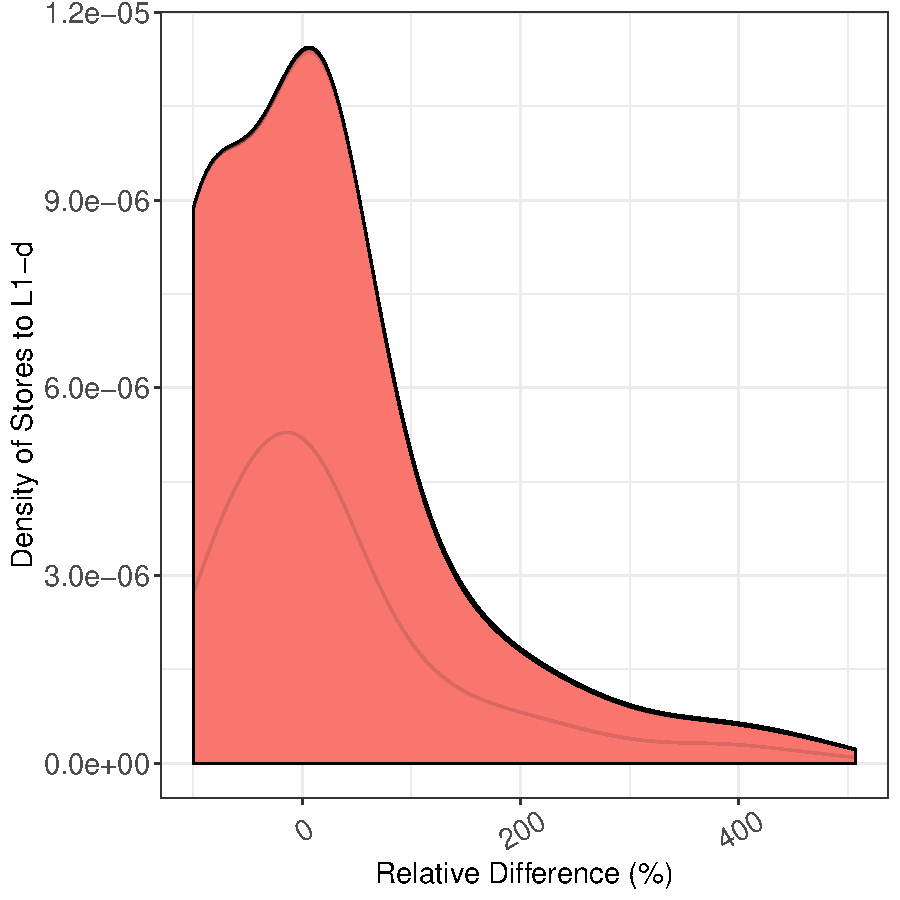
\includegraphics[scale=0.4]{graphs/kmeans/narrow_dist.pdf}
		\caption{Density of the fraction of approximateable stores within a store-value relative difference. Shown is focused view between relative percent difference of -500\% and 500\%.}
	\end{subfigure}
\caption{Kmeans} %need this for label to ref properly
\label{fig:kmeans_valsim}
\end{figure*}

\begin{figure*}[htbp]
	\begin{subfigure}{0.33\textwidth}
		\centering
		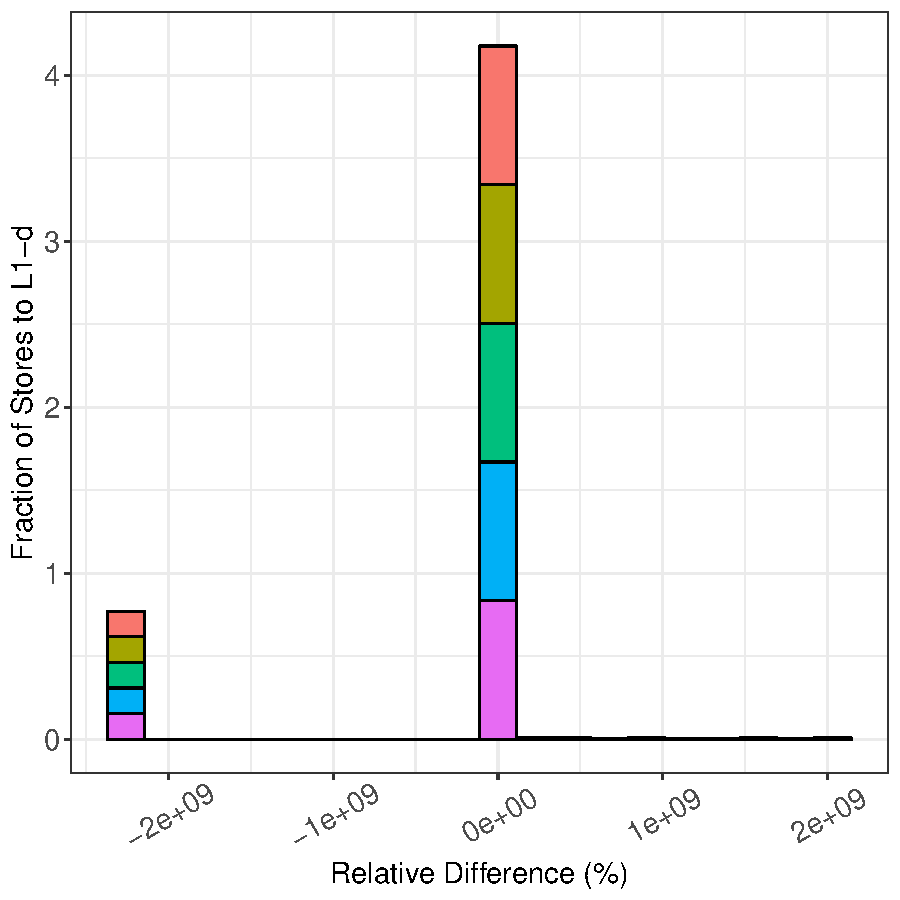
\includegraphics[scale=0.4]{graphs/kmeans_top5/full_hist.pdf}
		\caption{Histogram of the fraction of approximateable stores within a store-value relative difference. Shown is the full realtive difference range.}
	\end{subfigure}
	% Need a space between subfigures
	\begin{subfigure}{0.33\textwidth}
		\centering
		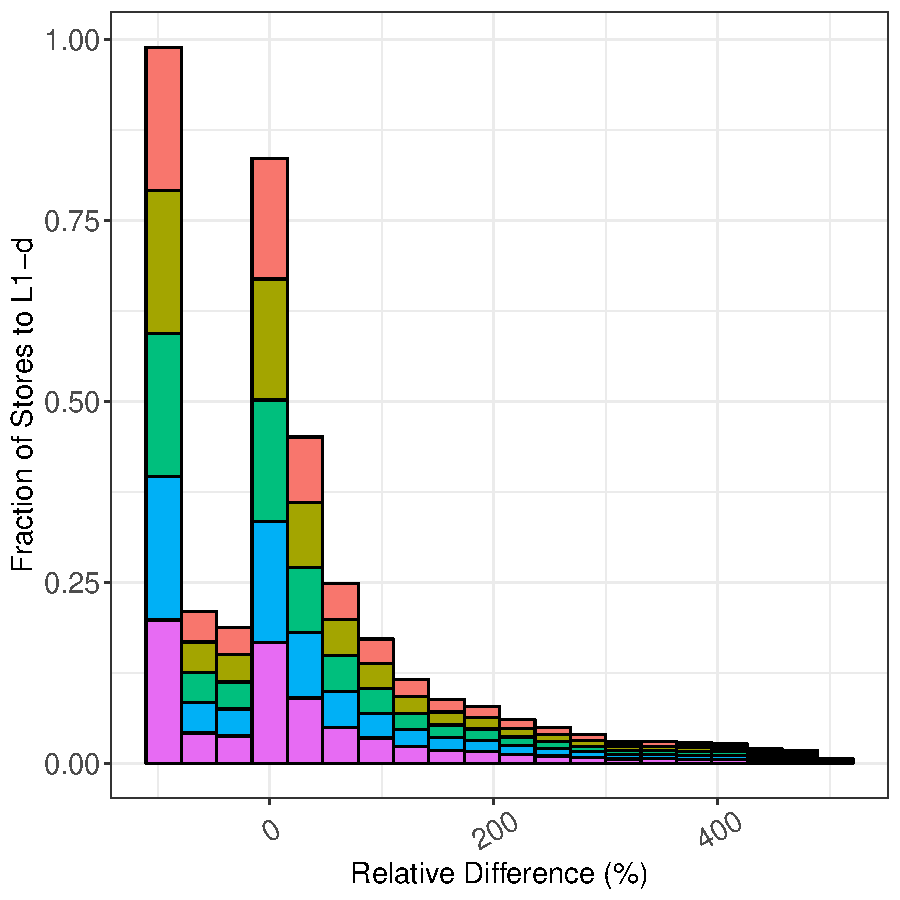
\includegraphics[scale=0.4]{graphs/kmeans_top5/narrow_hist.pdf}
		\caption{Histogram of the fraction of approximateable stores within a store-value relative difference. Shown is focused view between relative percent difference of -500\% and 500\%.}
	\end{subfigure}
	% Need a space between subfigures
	\begin{subfigure}{0.33\textwidth}
		\centering
		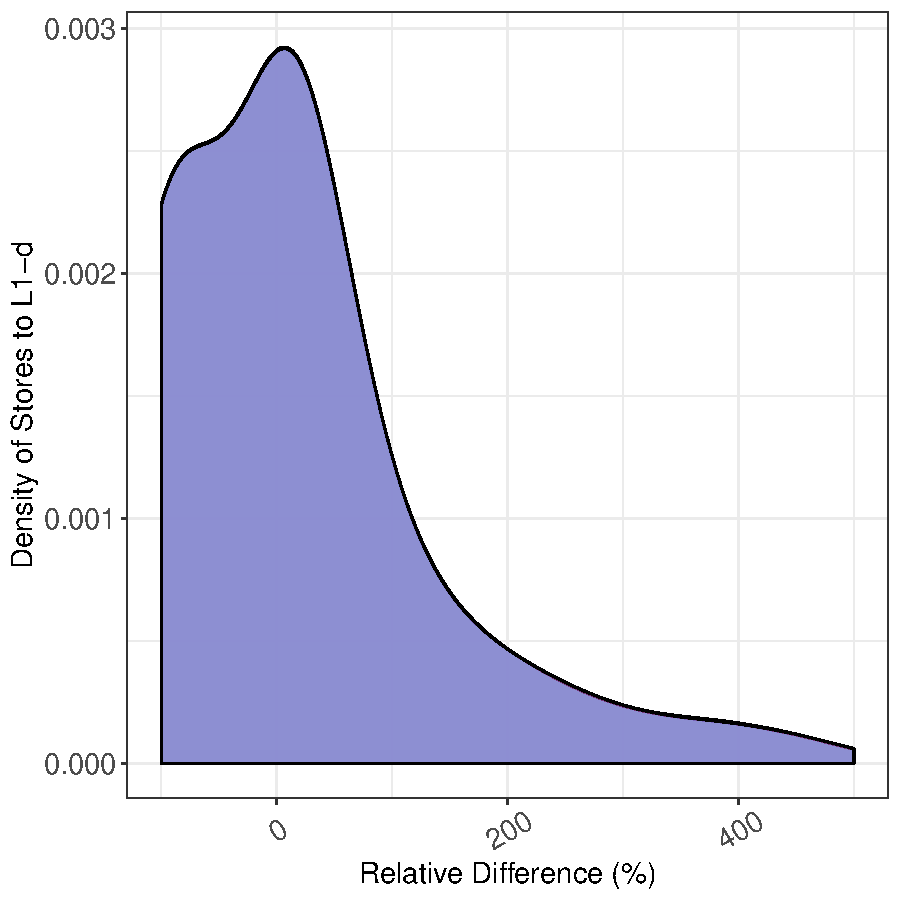
\includegraphics[scale=0.4]{graphs/kmeans_top5/narrow_dist.pdf}
		\caption{Density of the fraction of approximateable stores within a store-value relative difference. Shown is focused view between relative percent difference of -500\% and 500\%.}
	\end{subfigure}
\caption{KMeans top 5 stores} %need this for label to ref properly
\label{fig:kmeans_valsim_top5}
\end{figure*}



\begin{table}[htbp]
\caption{Stores saved for different level of approximations for benchmark KMeans}
	\begin{center}
		\begin{tabular}{|c|c|}
			\hline

			\textbf{Relative Difference (\%)} & \textbf{Stores Saved (\%)}\\
			\hline

			\textbf{1} & 4.86\\
			\hline

			\textbf{5} & 9.46\\
			\hline

			\textbf{10} & 13.14\\
			\hline

			\textbf{20} & 18.70\\
			\hline

			\textbf{30} & 22.94\\
			\hline

			\textbf{40} & 26.51\\
			\hline

			\textbf{50} & 30.25\\
			\hline

		\end{tabular}
	\label{tab:kmeans_reldiff}
	\end{center}
\end{table}


\begin{figure*}[htbp]
	\begin{subfigure}{0.33\textwidth}
		\centering
		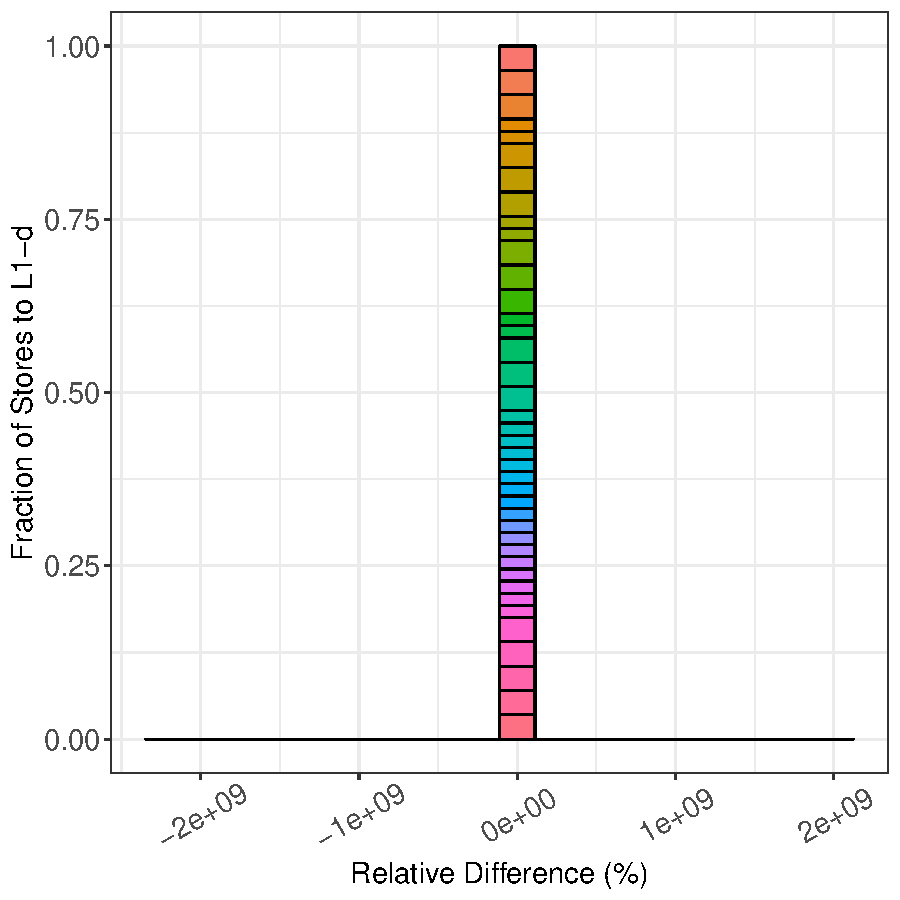
\includegraphics[scale=0.4]{graphs/linear_regression/full_hist.pdf}
		\caption{Histogram of the fraction of approximateable stores within a store-value relative difference. Shown is the full realtive difference range.}
	\end{subfigure}
	% Need a space between subfigures
	\begin{subfigure}{0.33\textwidth}
		\centering
		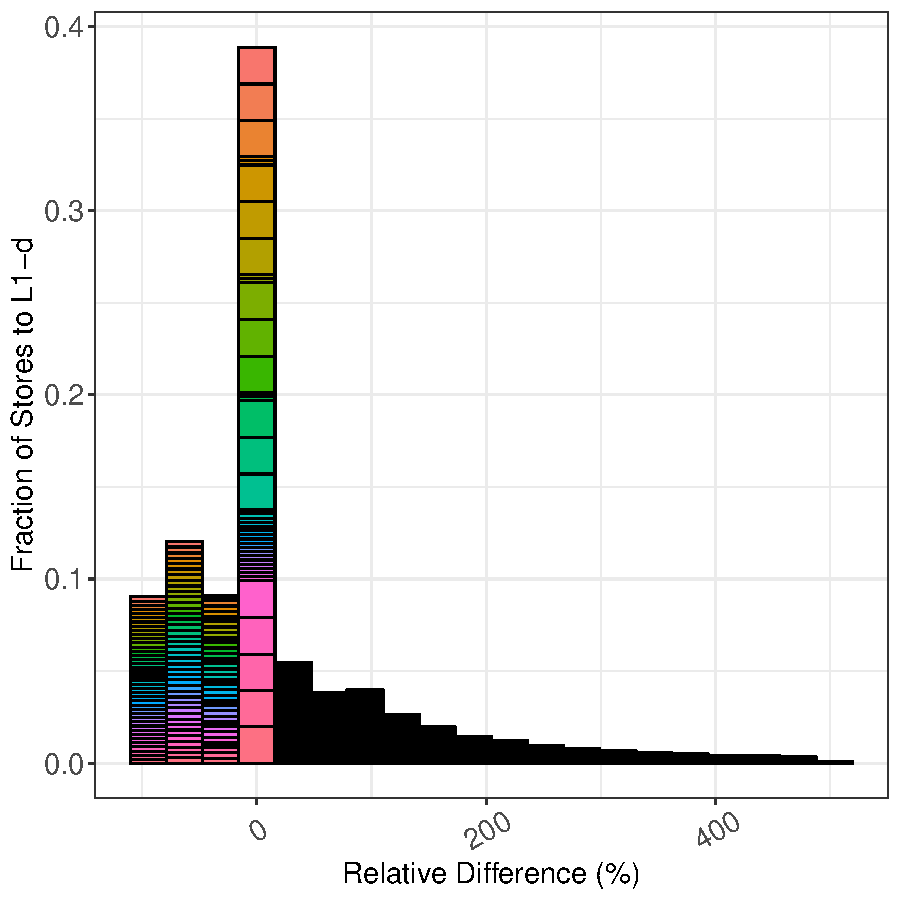
\includegraphics[scale=0.4]{graphs/linear_regression/narrow_hist.pdf}
		\caption{Histogram of the fraction of approximateable stores within a store-value relative difference. Shown is focused view between relative percent difference of -500\% and 500\%.}
	\end{subfigure}
	% Need a space between subfigures
	\begin{subfigure}{0.33\textwidth}
		\centering
		\includegraphics[scale=0.4]{graphs/linear_regression/narrow_dist.pdf}
		\caption{Density of the fraction of approximateable stores within a store-value relative difference. Shown is focused view between relative percent difference of -500\% and 500\%.}
	\end{subfigure}
\caption{Linear Regression} %need this for label to ref properly
\label{fig:linear_regression_valsim}
\end{figure*}

\begin{figure*}[htbp]
	\begin{subfigure}{0.33\textwidth}
		\centering
		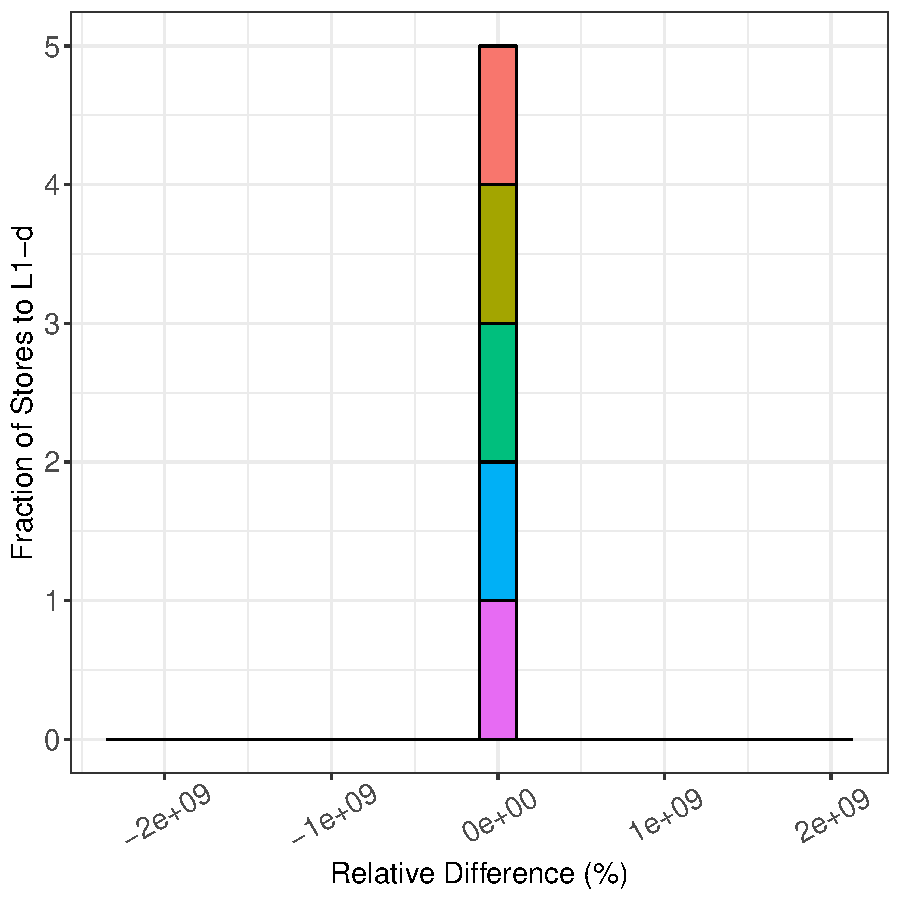
\includegraphics[scale=0.4]{graphs/linear_regression_top5/full_hist.pdf}
		\caption{Histogram of the fraction of approximateable stores within a store-value relative difference. Shown is the full realtive difference range.}
	\end{subfigure}
	% Need a space between subfigures
	\begin{subfigure}{0.33\textwidth}
		\centering
		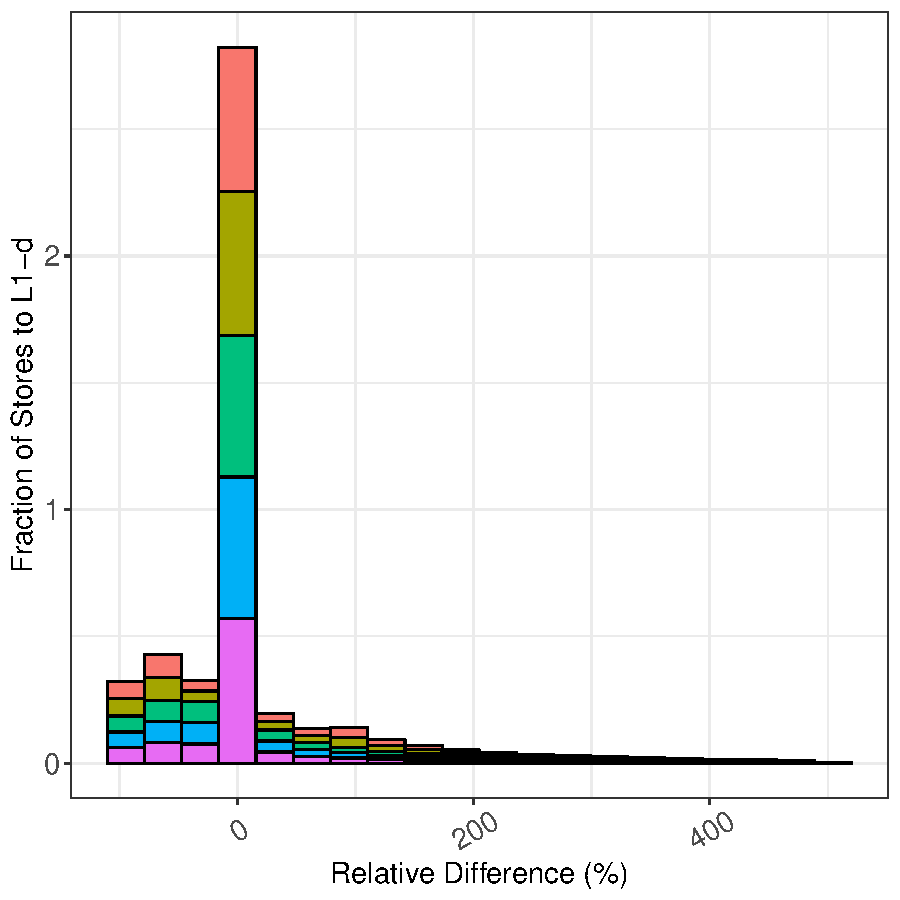
\includegraphics[scale=0.4]{graphs/linear_regression_top5/narrow_hist.pdf}
		\caption{Histogram of the fraction of approximateable stores within a store-value relative difference. Shown is focused view between relative percent difference of -500\% and 500\%.}
	\end{subfigure}
	% Need a space between subfigures
	\begin{subfigure}{0.33\textwidth}
		\centering
		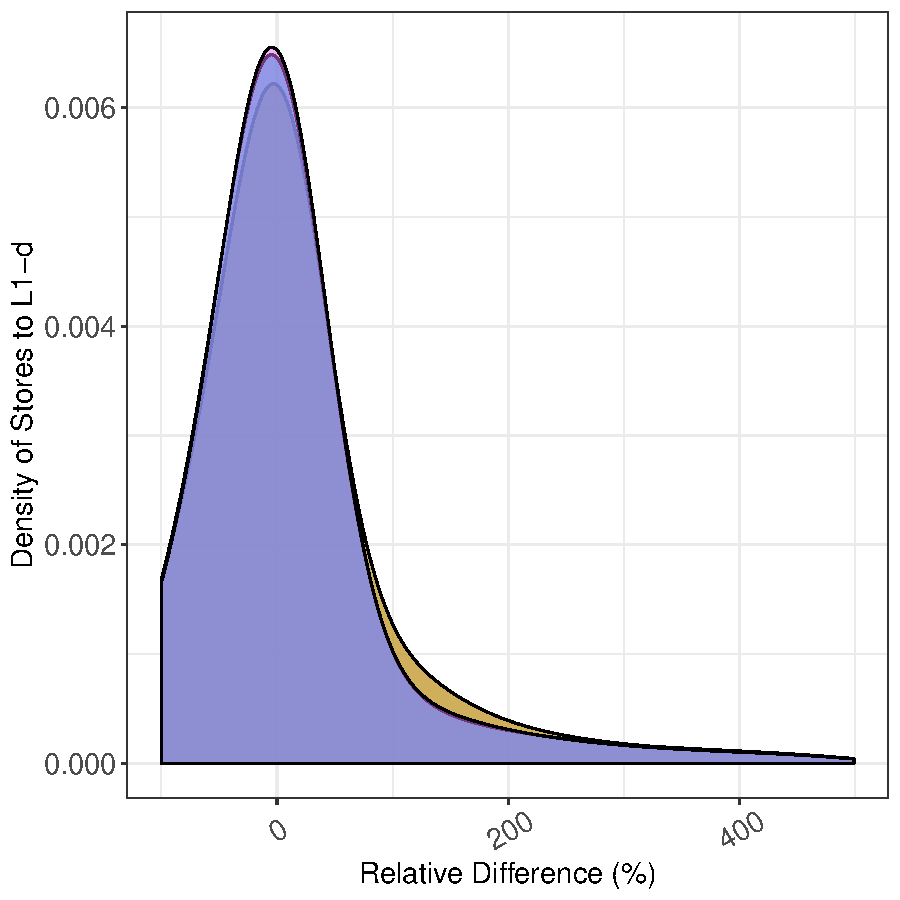
\includegraphics[scale=0.4]{graphs/linear_regression_top5/narrow_dist.pdf}
		\caption{Density of the fraction of approximateable stores within a store-value relative difference. Shown is focused view between relative percent difference of -500\% and 500\%.}
	\end{subfigure}
\caption{Linear Regression top 5 stores} %need this for label to ref properly
\label{fig:linear_regression_valsim_top5}
\end{figure*}




\begin{table}[htbp]
\caption{Stores saved for different level of approximations for benchmark Linear Regression}
	\begin{center}
		\begin{tabular}{|c|c|}
			\hline

			\textbf{Relative Difference (\%)} & \textbf{Stores Saved (\%)}\\
			\hline

			\textbf{1} & 50.50\\
			\hline

			\textbf{5} & 51.85\\
			\hline

			\textbf{10} & 54.27\\
			\hline

			\textbf{20} & 57.92\\
			\hline

			\textbf{30} & 61.21\\
			\hline

			\textbf{40} & 64.36\\
			\hline

			\textbf{50} & 67.49\\
			\hline

		\end{tabular}
	\label{tab:linear_regression_reldiff}
	\end{center}
\end{table}




\begin{figure*}[htbp]
	\begin{subfigure}{0.33\textwidth}
		\centering
		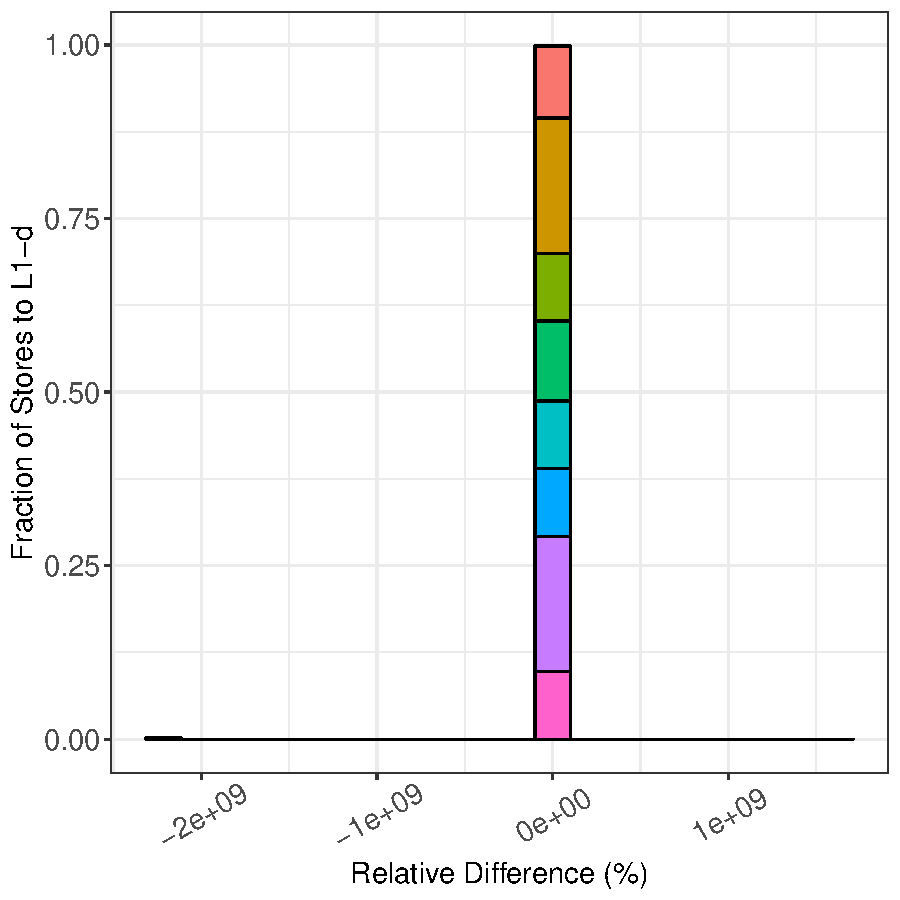
\includegraphics[scale=0.4]{graphs/matrix_multiply/full_hist.pdf}
		\caption{Histogram of the fraction of approximateable stores within a store-value relative difference. Shown is the full realtive difference range.}
	\end{subfigure}
	% Need a space between subfigures
	\begin{subfigure}{0.33\textwidth}
		\centering
		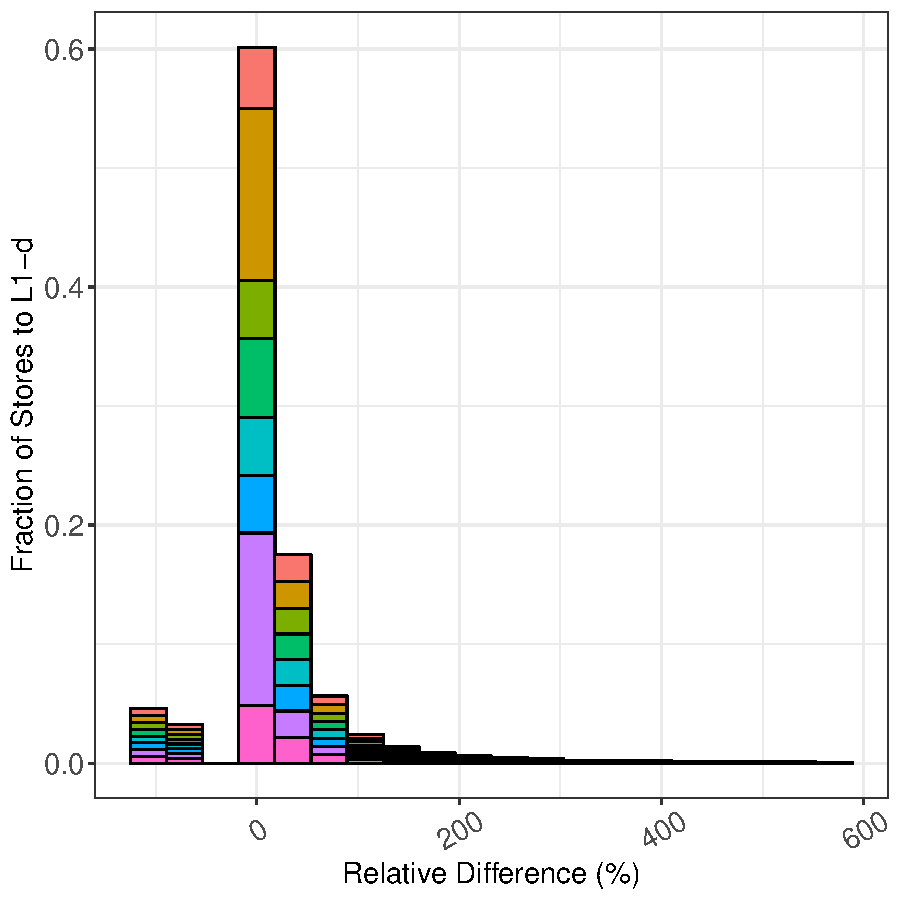
\includegraphics[scale=0.4]{graphs/matrix_multiply/narrow_hist.pdf}
		\caption{Histogram of the fraction of approximateable stores within a store-value relative difference. Shown is focused view between relative percent difference of -500\% and 500\%.}
	\end{subfigure}
	% Need a space between subfigures
	\begin{subfigure}{0.33\textwidth}
		\centering
		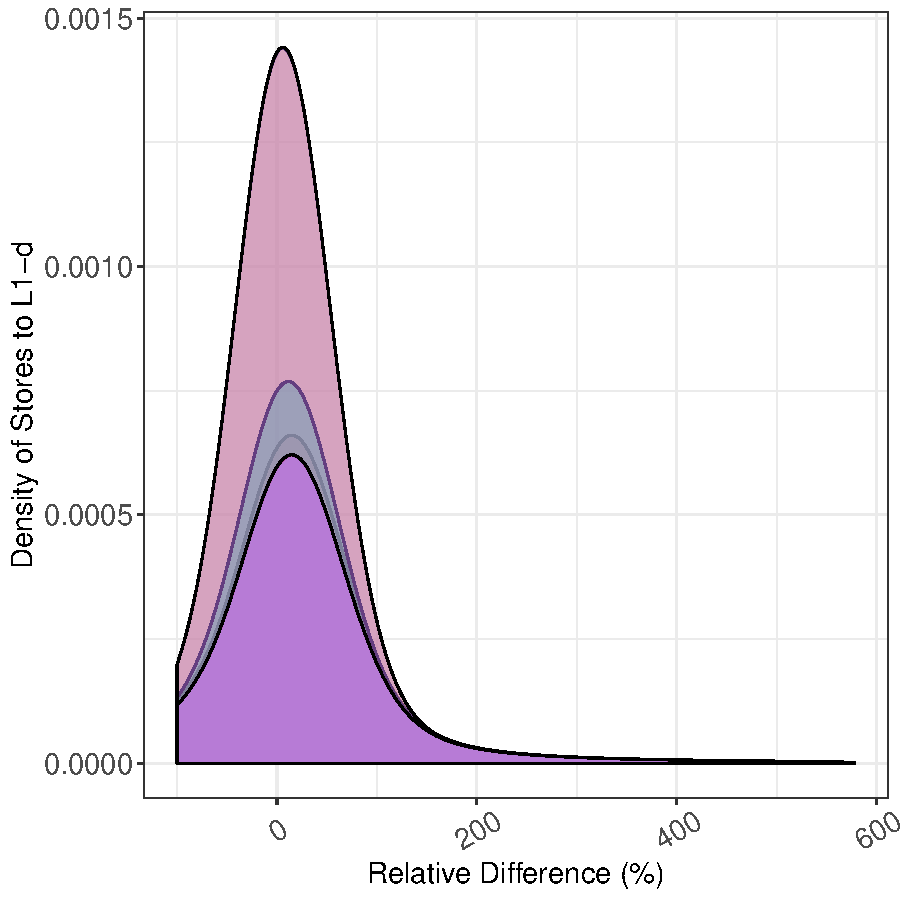
\includegraphics[scale=0.4]{graphs/matrix_multiply/narrow_dist.pdf}
		\caption{Density of the fraction of approximateable stores within a store-value relative difference. Shown is focused view between relative percent difference of -500\% and 500\%.}
	\end{subfigure}
\caption{Matrix Multiply} %need this for label to ref properly
\label{fig:matrix_multiply_valsim}
\end{figure*}

\begin{figure*}[htbp]
	\begin{subfigure}{0.33\textwidth}
		\centering
		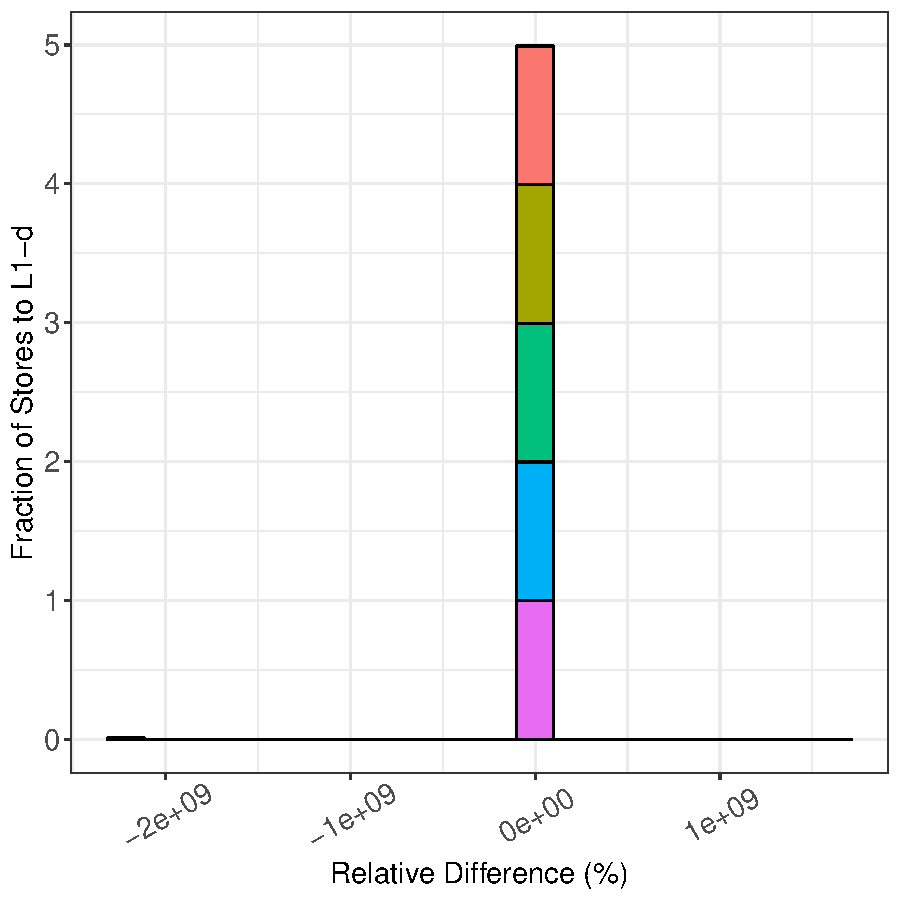
\includegraphics[scale=0.4]{graphs/matrix_multiply_top5/full_hist.pdf}
		\caption{Histogram of the fraction of approximateable stores within a store-value relative difference. Shown is the full realtive difference range.}
	\end{subfigure}
	% Need a space between subfigures
	\begin{subfigure}{0.33\textwidth}
		\centering
		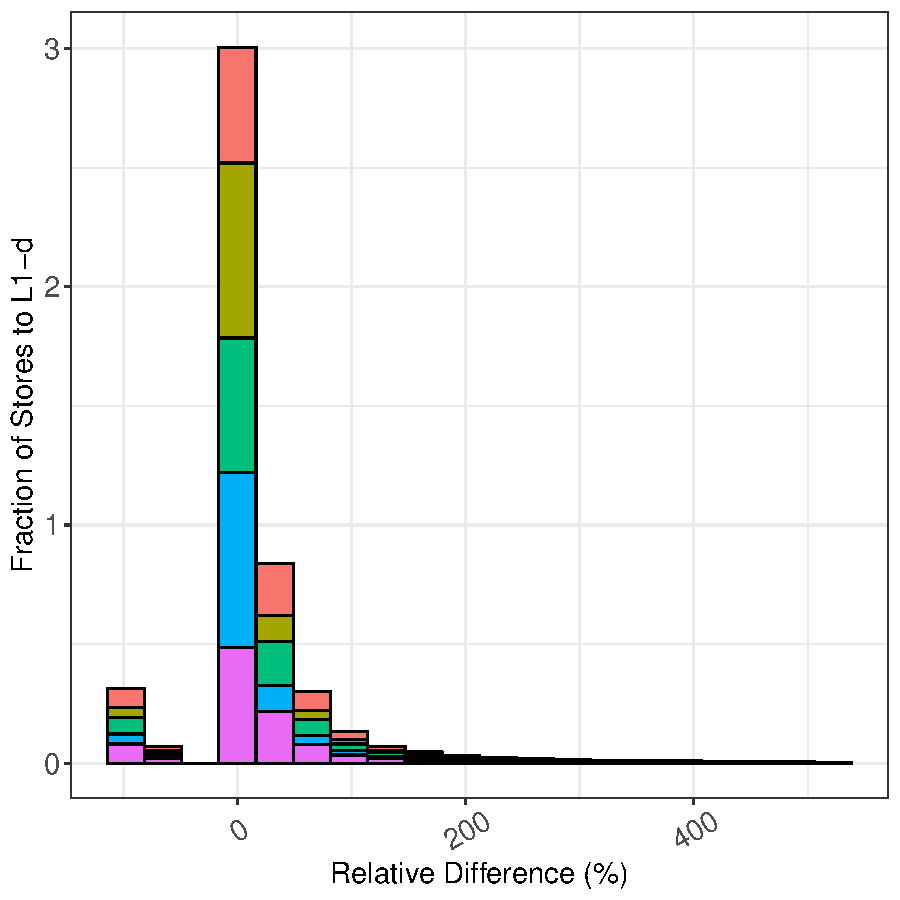
\includegraphics[scale=0.4]{graphs/matrix_multiply_top5/narrow_hist.pdf}
		\caption{Histogram of the fraction of approximateable stores within a store-value relative difference. Shown is focused view between relative percent difference of -500\% and 500\%.}
	\end{subfigure}
	% Need a space between subfigures
	\begin{subfigure}{0.33\textwidth}
		\centering
		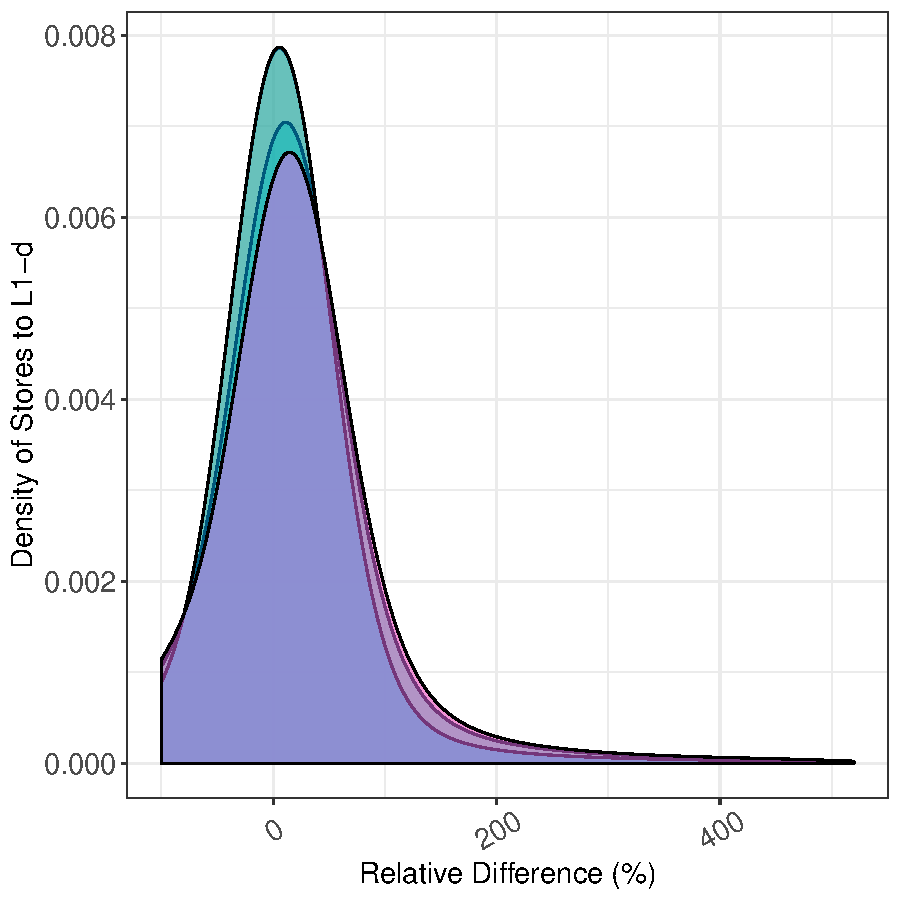
\includegraphics[scale=0.4]{graphs/matrix_multiply_top5/narrow_dist.pdf}
		\caption{Density of the fraction of approximateable stores within a store-value relative difference. Shown is focused view between relative percent difference of -500\% and 500\%.}
	\end{subfigure}
\caption{Matrix Multiply top 5 stores} %need this for label to ref properly
\label{fig:matrix_multiply_valsim_top5}
\end{figure*}




\begin{table}[htbp]
\caption{Stores saved for different level of approximations for benchmark Matrix Multiply}
	\begin{center}
		\begin{tabular}{|c|c|}
			\hline

			\textbf{Relative Difference (\%)} & \textbf{Stores Saved (\%)}\\
			\hline

			\textbf{1} & 36.68\\
			\hline

			\textbf{5} & 48.46\\
			\hline

			\textbf{10} & 56.32\\
			\hline

			\textbf{20} & 66.09\\
			\hline

			\textbf{30} & 72.12\\
			\hline

			\textbf{40} & 76.28\\
			\hline

			\textbf{50} & 79.25\\
			\hline

		\end{tabular}
	\label{tab:matrix_multiply_reldiff}
	\end{center}
\end{table}




\begin{figure*}[htbp]
	\begin{subfigure}{0.33\textwidth}
		\centering
		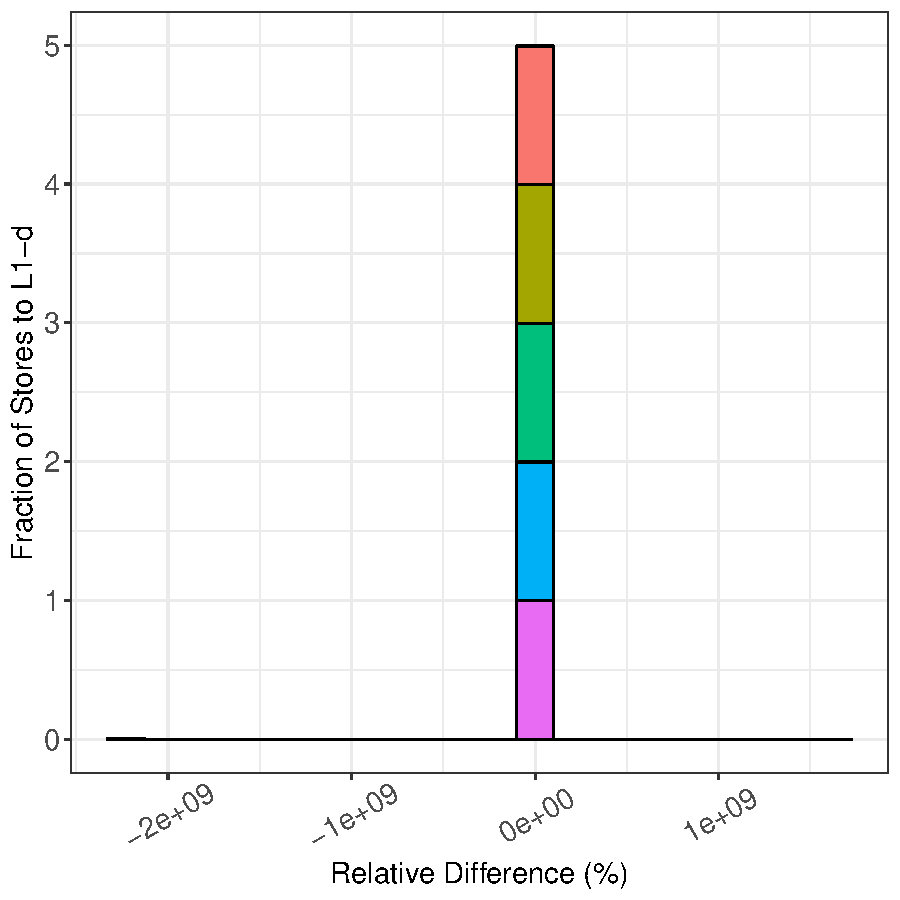
\includegraphics[scale=0.4]{graphs/pca_top5/full_hist.pdf}
		\caption{Histogram of the fraction of approximateable stores within a store-value relative difference. Shown is the full realtive difference range.}
	\end{subfigure}
	% Need a space between subfigures
	\begin{subfigure}{0.33\textwidth}
		\centering
		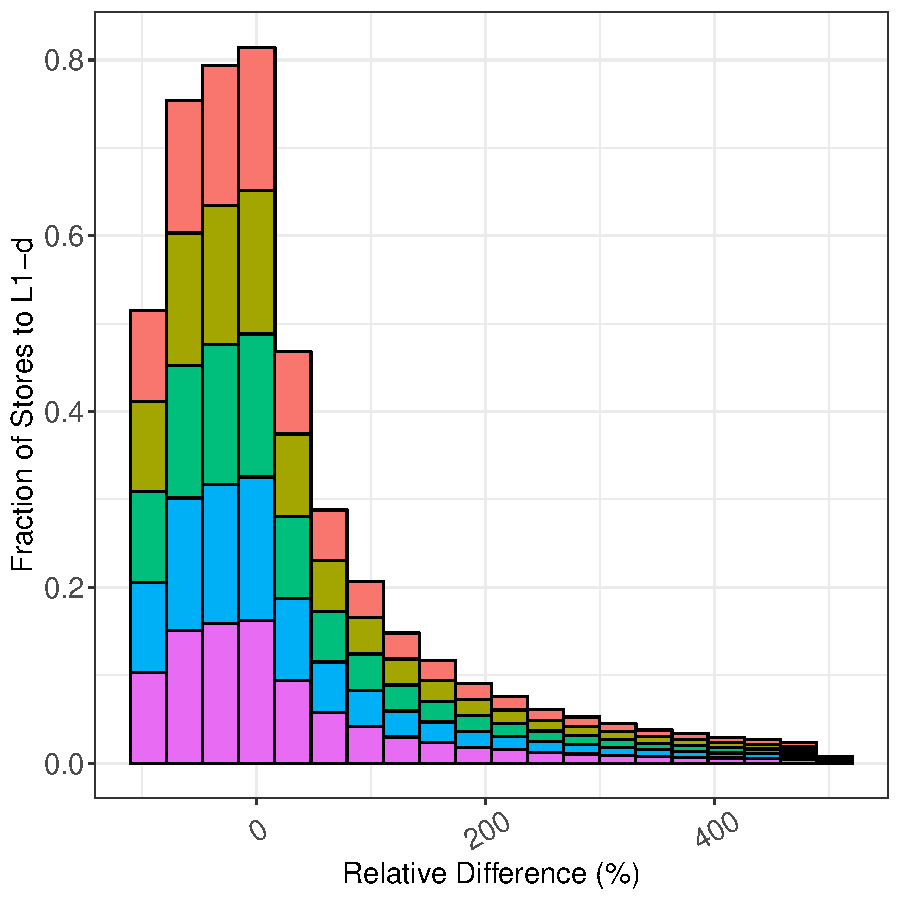
\includegraphics[scale=0.4]{graphs/pca_top5/narrow_hist.pdf}
		\caption{Histogram of the fraction of approximateable stores within a store-value relative difference. Shown is focused view between relative percent difference of -500\% and 500\%.}
	\end{subfigure}
	% Need a space between subfigures
	\begin{subfigure}{0.33\textwidth}
		\centering
		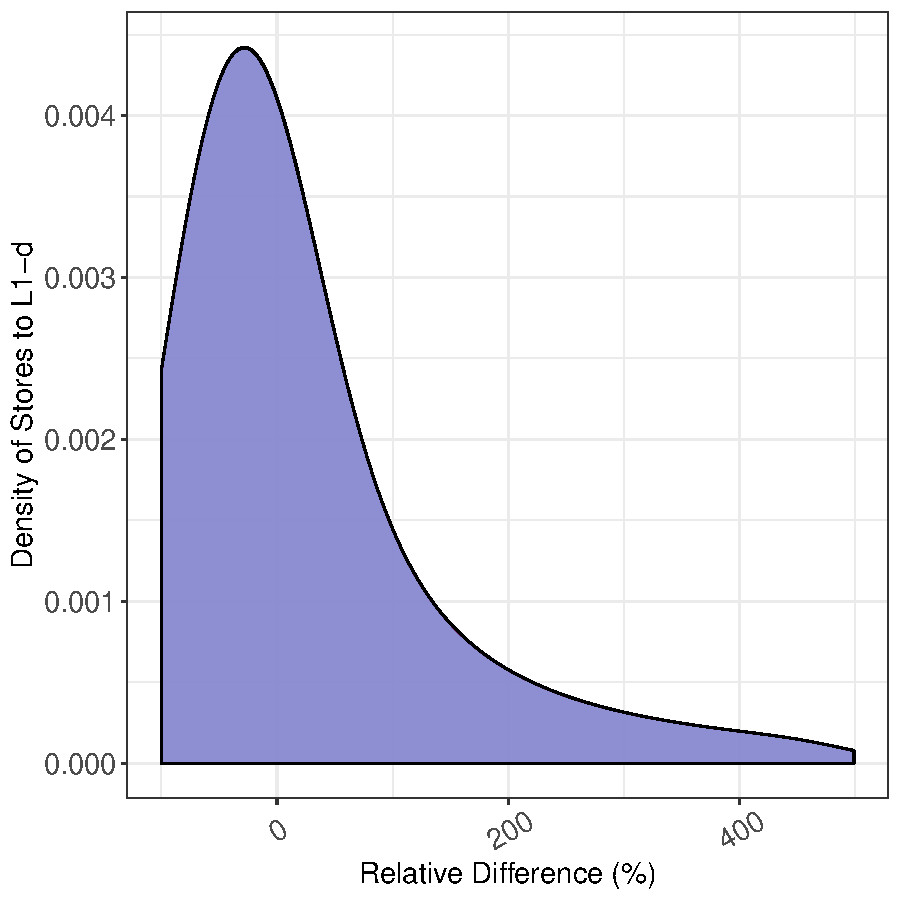
\includegraphics[scale=0.4]{graphs/pca_top5/narrow_dist.pdf}
		\caption{Density of the fraction of approximateable stores within a store-value relative difference. Shown is focused view between relative percent difference of -500\% and 500\%.}
	\end{subfigure}
\caption{PCA top 5 stores} %need this for label to ref properly
\label{fig:pca_valsim_top5}
\end{figure*}


\begin{table}[htbp]
\caption{Stores saved for different level of approximations for benchmark PCA}
	\begin{center}
		\begin{tabular}{|c|c|}
			\hline

			\textbf{Relative Difference (\%)} & \textbf{Stores Saved (\%)}\\
			\hline

			\textbf{1} & 3.00\\
			\hline

			\textbf{5} & 6.22\\
			\hline

			\textbf{10} & 10.91\\
			\hline

			\textbf{20} & 19.78\\
			\hline

			\textbf{30} & 28.02\\
			\hline

			\textbf{40} & 35.69\\
			\hline

			\textbf{50} & 42.93\\
			\hline

		\end{tabular}
	\label{tab:pca_reldiff}
	\end{center}
\end{table}




% \subsection*{Silent Approximate Stores}

% \begin{table}[htbp]
% \caption{Table Type Styles}
% 	\begin{center}
% 		\begin{tabular}{|c|c|c|c|}
% 			\hline
% 			% \textbf{Table}&\multicolumn{3}{|c|}{\textbf{Table Column Head}} \\
% 			% \cline{2-4} 
% 			\textbf{Benchmark} & \textbf{Approximation \%}& \textbf{Traffic Reduced \%} & \textbf{NRMSE \%}\\
% 			\hline

% 			\multirow{3}{*}{\textbf{Histogram}} & 5 & & 5.36 \\
% 			 & 10 & & 5.40 \\
% 			 & 25 &  & 5.32 \\
% 			\hline

% 			\multirow{3}{*}{\textbf{KMeans}} & 5 & 88.58 & 1.44 \\
% 			 & 10 & 90.30  & 2.63 \\
% 			 & 25 & 91.60 & 2.63 \\
% 			\hline

% 			\multirow{3}{*}{\textbf{PCA}} & 5 & 44.77 & 96.59 \\
% 			 & 10 & 47.98 & 121.51\\
% 			 & 25 & 48.80 & 121.54\\
% 			\hline

% 		\end{tabular}
% 	\label{tab1}
% 	\end{center}
% \end{table}

% Hopefully I'll have a table here how much SAS can reduce coherence traffic based on approximation percentage.

% Tie this in with Store-value similarity how we can mitigate some of the effects of the traffic caused by silent stores by keep in line in Shared state. SAS on invalid lines from false sharing by not acutally storing can also help save traffic.